\documentclass[12pt, a4paper]{article}

% Packages
\usepackage[margin=1in]{geometry}
\usepackage{graphicx}
\usepackage{booktabs}
\usepackage{hyperref}
\usepackage{amsmath}
\usepackage{enumitem}
\usepackage{caption}
\usepackage{subcaption}
\usepackage{xcolor}
\usepackage{titlesec}
\usepackage{setspace}
\usepackage[numbers]{natbib}
\usepackage{multirow}
\usepackage{array}
\usepackage{tikz}
\usetikzlibrary{shapes.geometric, arrows.meta, positioning, fit, backgrounds}

% Formatting
\onehalfspacing
\titleformat{\section}{\large\bfseries}{\thesection.}{0.5em}{}
\titleformat{\subsection}{\normalsize\bfseries}{\thesubsection}{0.5em}{}

\hypersetup{
    colorlinks=true,
    linkcolor=blue,
    citecolor=blue,
    urlcolor=blue
}

\begin{document}

% ============ TITLE PAGE ============
\begin{center}
    {\large \textbf{National Institute of Technology Calicut}}\\[0.3cm]
    {\normalsize Department of Computer Science \& Engineering}\\[1.5cm]
    
    {\Large \textbf{Weekly Progress Report --- Week 2}}\\[0.8cm]
    
    {\LARGE \textbf{Architectural Analysis of Domain-Adaptive\\[0.3cm] Video Anomaly Detection Frameworks}}\\[1.5cm]
    
    {\large Follow-up to: Domain Adaptability Literature Review (Week 1)}\\[1.5cm]
    
    \begin{tabular}{rl}
        \textbf{Student:} & [Your Name] \\
        \textbf{Roll No:} & [Your Roll Number] \\
        \textbf{Guide:} & Prof.\ [Professor Name] \\
        \textbf{Date:} & \today \\
    \end{tabular}
\end{center}

\newpage

% ============ 1. SUMMARY OF PROGRESS ============
\section{Summary of This Week's Progress}

Following last week's literature review of the ``Quo Vadis'' survey (arXiv:2412.18298) and the identification of OVVAD, VERA, and LAVAD as the three most relevant frameworks, this week's work focused on:

\begin{enumerate}[leftmargin=*]
    \item \textbf{Deep architectural analysis} of the three identified papers --- studying their full manuscripts, not just the survey summaries --- to extract exact design choices, module specifications, and training paradigms.
    \item \textbf{Comparative evaluation} across architectural dimensions (backbone, temporal modeling, domain adaptation mechanism, training requirement, and reported performance).
    \item \textbf{Designing a unified architecture proposal} that synthesizes the strongest components from each framework into a cohesive pipeline for our project.
    \item \textbf{Environment setup and feasibility verification} --- confirming software compatibility, GPU memory requirements, and dataset accessibility for the planned experiments.
\end{enumerate}

% ============ 2. DETAILED ARCHITECTURAL ANALYSIS ============
\section{Detailed Architectural Analysis of Identified Frameworks}

Each of the three papers identified in last week's report was studied in full. The following subsections detail the precise architectural components and design rationale of each.

\subsection{OVVAD --- Open-Vocabulary Video Anomaly Detection \cite{wu2024ovvad}}

\textbf{Venue:} CVPR 2024 \hfill \textbf{Setting:} Weakly Supervised, Open-Vocabulary

OVVAD decouples the video anomaly detection problem into two complementary sub-tasks: (i) \textit{class-agnostic detection} --- binary normal/abnormal classification, and (ii) \textit{class-specific categorization} --- recognizing both seen (base) and unseen (novel) anomaly types.

\begin{itemize}[leftmargin=*]
    \item \textbf{Visual Backbone:} Frozen CLIP ViT-B/16 image encoder. Frame-level features are extracted without any fine-tuning of the vision encoder, preserving its zero-shot generalization capability.
    
    \item \textbf{Temporal Adapter (TA):} A lightweight, nearly weight-free temporal adapter module is placed on top of the frozen CLIP features. This module captures inter-frame temporal dependencies while deliberately avoiding overfitting to the source domain's visual distribution.
    
    \item \textbf{Semantic Knowledge Injection (SKI):} An auxiliary module that injects external textual knowledge (generated via LLMs or category descriptions) into the visual feature pipeline. This bridges the semantic gap between visual representations and open-vocabulary anomaly categories.
    
    \item \textbf{Anomaly Synthesis:} Pseudo-novel anomaly videos are synthesized during training to expose the model to unseen anomaly categories, enabling generalization beyond the labeled training set.
    
    \item \textbf{Reported Performance:} 86.40\% AUC on UCF-Crime dataset.
\end{itemize}

\textbf{Key Takeaway for Our Project:} The frozen encoder + lightweight temporal adapter paradigm is highly relevant. It demonstrates that temporal modeling can be added \textit{on top of} a pretrained VLM without compromising its domain-agnostic capabilities.

\subsection{LAVAD --- Harnessing LLMs for Training-Free VAD \cite{zanella2024lavad}}

\textbf{Venue:} CVPR 2024 \hfill \textbf{Setting:} Fully Training-Free

LAVAD introduces a ``caption-then-reason'' pipeline that requires \textbf{zero training} --- no fine-tuning, no learned modules, and no domain-specific data collection.

\begin{itemize}[leftmargin=*]
    \item \textbf{Frame Captioning:} A pretrained Vision-Language Model (BLIP-2) generates dense textual descriptions for each video frame, converting the visual stream into a sequence of natural language captions.
    
    \item \textbf{Temporal Aggregation:} Captions from temporally adjacent frames are grouped into snippets. An LLM is queried with these caption sequences to produce a ``temporal summary'' that captures dynamic scene evolution across the snippet window.
    
    \item \textbf{Anomaly Scoring via LLM:} The LLM is prompted to assign an anomaly score (0--1) to each temporal summary based on semantic reasoning. This bypasses traditional learned scoring heads entirely.
    
    \item \textbf{Cross-Modal Refinement:} To mitigate noisy or hallucinated captions, LAVAD employs a cross-modal similarity mechanism using video-text embeddings to refine the LLM-generated scores, ensuring only semantically consistent frames contribute to the final prediction.
    
    \item \textbf{Reported Performance:} Outperforms all unsupervised and one-class VAD methods on UCF-Crime (+6.08\% over GCL, +0.52\% over DyAnNet) without any training.
\end{itemize}

\textbf{Key Takeaway for Our Project:} LAVAD validates the hypothesis that an LLM can serve as the reasoning engine for anomaly detection through language alone. The cross-modal refinement step is critical --- raw VLM captions are noisy and require grounding against visual features for reliable scoring.

\subsection{VERA --- Explainable VAD via Verbalized Learning \cite{ye2025vera}}

\textbf{Venue:} CVPR 2025 \hfill \textbf{Setting:} Training-Free, Explainable

VERA extends the training-free paradigm by introducing \textit{verbalized learning} --- the model's understanding of normality is expressed and manipulated entirely through natural language, enabling dynamic domain adaptation at inference time.

\begin{itemize}[leftmargin=*]
    \item \textbf{Verbalized Context Prompting:} Instead of training domain-specific features, VERA verbalizes the deployment context directly into the VLM's text prompt (e.g., \textit{``A dimly lit warehouse corridor with conveyor belts''}). This dynamically adjusts the model's baseline of normality to the target domain.
    
    \item \textbf{Scene-Adaptive Reasoning:} The VLM reasons about anomalies \textit{relative to the verbalized context}, making detection inherently domain-adaptive. A ``running person'' may be normal in a sports arena but anomalous in a restricted warehouse --- VERA handles this distinction through prompt context alone.
    
    \item \textbf{Explainability:} Every detection is accompanied by a natural language explanation grounded in the verbalized context, providing auditable reasoning chains for industrial deployment.
    
    \item \textbf{Cross-Domain Robustness:} VERA demonstrates high robustness when transferred across domains (surveillance $\rightarrow$ industrial, indoor $\rightarrow$ outdoor) without any parameter changes, confirming the power of verbalized domain descriptions.
\end{itemize}

\textbf{Key Takeaway for Our Project:} Verbalized prompting is the most elegant mechanism for domain adaptation in our zero-shot pipeline. It eliminates the need for even lightweight adapter training when switching domains, requiring only a textual description of the new deployment environment.

% ============ 3. COMPARATIVE ANALYSIS TABLE ============
\section{Comparative Architectural Analysis}

Table~\ref{tab:comparison} presents a structured comparison of the three frameworks across key architectural dimensions relevant to our project requirements.

\begin{table}[h!]
\centering
\caption{Comparative Analysis of OVVAD, LAVAD, and VERA}
\label{tab:comparison}
\renewcommand{\arraystretch}{1.35}
\small
\begin{tabular}{@{} p{2.8cm} p{3.8cm} p{3.8cm} p{3.8cm} @{}}
\toprule
\textbf{Dimension} & \textbf{OVVAD (CVPR '24)} & \textbf{LAVAD (CVPR '24)} & \textbf{VERA (CVPR '25)} \\
\midrule
\textbf{Visual Backbone} & Frozen CLIP ViT-B/16 & BLIP-2 (captioning) & VLM (frozen) \\
\addlinespace
\textbf{Temporal Modeling} & Lightweight Temporal Adapter (learned) & LLM temporal aggregation over caption sequences & Implicit via multi-frame verbalized prompts \\
\addlinespace
\textbf{Domain Adaptation} & Semantic Knowledge Injection + Anomaly Synthesis & Fully handled by LLM reasoning (no adaptation module) & Verbalized context prompting at inference \\
\addlinespace
\textbf{Anomaly Scoring} & Learned classifier head & LLM-assigned scores (0--1) + cross-modal refinement & VLM reasoning with context-relative scoring \\
\addlinespace
\textbf{Training Required?} & Yes (weakly supervised) & \textbf{No} (fully training-free) & \textbf{No} (fully training-free) \\
\addlinespace
\textbf{Explainability} & No (score only) & Partial (temporal summaries) & \textbf{Yes} (full natural language) \\
\addlinespace
\textbf{Open-Vocabulary?} & Yes (base + novel) & Implicitly (via language) & Implicitly (via language) \\
\addlinespace
\textbf{Key Strength} & Strong temporal features with minimal overhead & Zero training, LLM-powered reasoning & Domain-adaptive + explainable \\
\addlinespace
\textbf{Key Weakness} & Requires training data; no explanations & Noisy captions; LLM cost & Less explored quantitatively \\
\bottomrule
\end{tabular}
\end{table}

% ============ 4. PROPOSED UNIFIED ARCHITECTURE ============
\section{Proposed Unified Architecture}

Based on the comparative analysis, we propose a unified architecture that selectively combines the strongest elements of each framework. The design philosophy is: \textit{maximize domain adaptability and explainability while maintaining a training-free core, with an optional lightweight adapter for temporal enhancement.}

\subsection{Architecture Overview}

The proposed pipeline, which we tentatively name \textbf{DA-ZVAD} (\textbf{D}omain-\textbf{A}daptive \textbf{Z}ero-shot \textbf{V}ideo \textbf{A}nomaly \textbf{D}etection), consists of four modules:

\begin{figure}[h!]
\centering
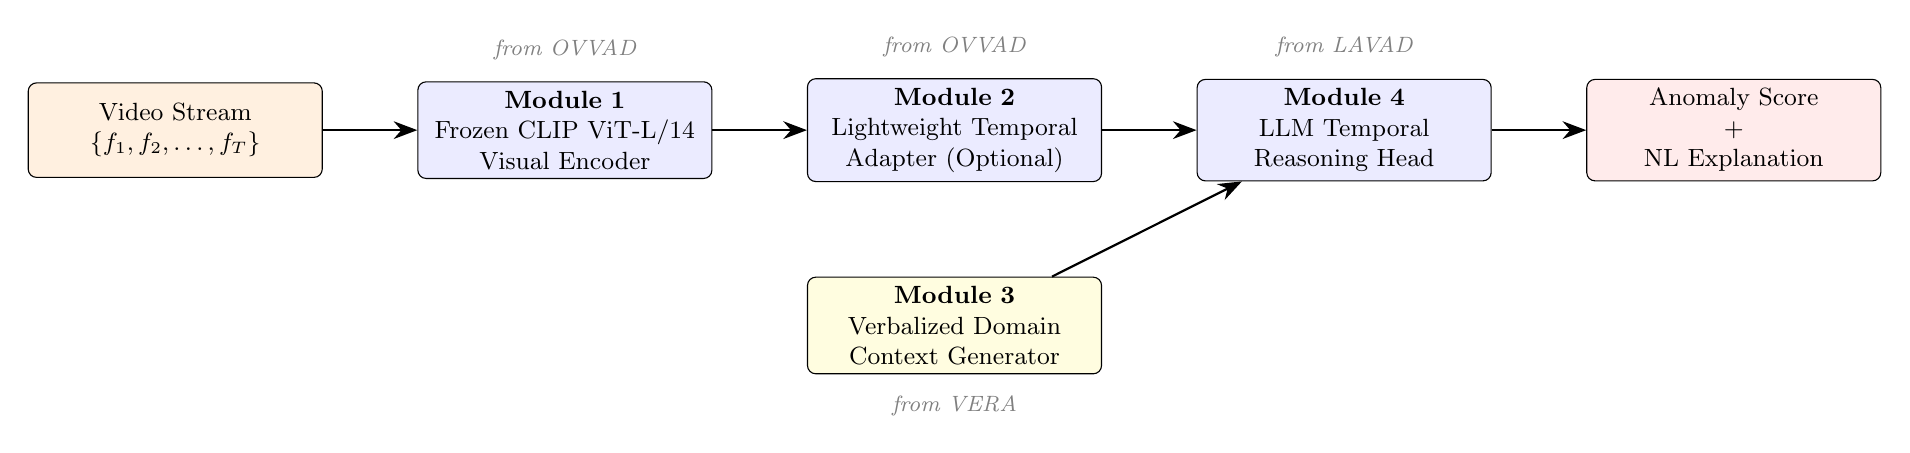
\begin{tikzpicture}[
    node distance=0.6cm and 1.2cm,
    block/.style={rectangle, draw, fill=blue!8, text width=3.5cm, minimum height=1.2cm, align=center, rounded corners=3pt, font=\small},
    smallblock/.style={rectangle, draw, fill=green!8, text width=3cm, minimum height=0.9cm, align=center, rounded corners=3pt, font=\footnotesize},
    arrow/.style={-{Stealth[length=3mm]}, thick},
    label/.style={font=\footnotesize\itshape, text=gray}
]

% Input
\node[block, fill=orange!12] (input) {Video Stream\\$\{f_1, f_2, \ldots, f_T\}$};

% Module 1: Visual Encoder
\node[block, right=of input] (encoder) {\textbf{Module 1}\\Frozen CLIP ViT-L/14\\Visual Encoder};

% Module 2: Temporal Adapter
\node[block, right=of encoder] (temporal) {\textbf{Module 2}\\Lightweight Temporal\\Adapter (Optional)};

% Module 3: Verbalized Context (below)
\node[block, below=1.2cm of temporal, fill=yellow!12] (verbal) {\textbf{Module 3}\\Verbalized Domain\\Context Generator};

% Module 4: LLM Reasoning
\node[block, right=of temporal] (llm) {\textbf{Module 4}\\LLM Temporal\\Reasoning Head};

% Output
\node[block, right=of llm, fill=red!8] (output) {Anomaly Score\\+\\NL Explanation};

% Arrows
\draw[arrow] (input) -- (encoder);
\draw[arrow] (encoder) -- (temporal);
\draw[arrow] (temporal) -- (llm);
\draw[arrow] (verbal) -- (llm);
\draw[arrow] (llm) -- (output);

% Labels
\node[label, above=0.15cm of encoder] {from OVVAD};
\node[label, above=0.15cm of temporal] {from OVVAD};
\node[label, below=0.15cm of verbal] {from VERA};
\node[label, above=0.15cm of llm] {from LAVAD};

\end{tikzpicture}
\caption{Proposed DA-ZVAD architecture combining elements from OVVAD, LAVAD, and VERA.}
\label{fig:architecture}
\end{figure}

\subsection{Module Descriptions}

\begin{enumerate}[leftmargin=*]
    \item \textbf{Module 1 --- Frozen Visual Encoder (from OVVAD):} 
    A frozen CLIP ViT-L/14 encoder extracts frame-level visual features. We choose ViT-L/14 over ViT-B/16 (used in OVVAD) for its superior representational capacity, which is critical given that we will not be fine-tuning the encoder. The frozen encoder ensures that the model's generalization to unseen domains is preserved.
    
    \item \textbf{Module 2 --- Lightweight Temporal Adapter (from OVVAD):} 
    An optional, nearly weight-free temporal adapter captures inter-frame dynamics. In the fully zero-shot configuration, this module is bypassed (features are passed directly to Module 4). When few-shot domain-specific data is available, this module can be trained to capture domain-specific temporal patterns with minimal parameters ($<$1M), following OVVAD's design.
    
    \item \textbf{Module 3 --- Verbalized Domain Context Generator (from VERA):} 
    This module generates a natural language description of the deployment domain. It operates in two modes:
    \begin{itemize}
        \item \textit{Manual mode:} The operator provides a textual description (e.g., ``Night-shift assembly line in an automotive welding station'').
        \item \textit{Automatic mode:} A VLM analyzes the first $N$ frames and generates a scene description automatically, enabling fully autonomous deployment.
    \end{itemize}
    The generated context is injected into the LLM reasoning prompt, grounding all anomaly assessments within the specific domain context.
    
    \item \textbf{Module 4 --- LLM Temporal Reasoning Head (from LAVAD):} 
    An LLM receives: (a) temporally aggregated visual features or frame captions, (b) the verbalized domain context from Module 3, and (c) a structured prompt requesting anomaly scoring and explanation. The LLM outputs both a numerical anomaly score and a natural language explanation. Cross-modal refinement (per LAVAD) is applied to suppress hallucinated or noisy predictions.
\end{enumerate}

\subsection{Operating Modes}

The architecture supports three deployment configurations:

\begin{table}[h!]
\centering
\caption{DA-ZVAD Operating Modes}
\label{tab:modes}
\renewcommand{\arraystretch}{1.3}
\begin{tabular}{@{} l c c c l @{}}
\toprule
\textbf{Mode} & \textbf{Module 2} & \textbf{Module 3} & \textbf{Training} & \textbf{Use Case} \\
\midrule
Zero-Shot & Bypassed & Auto/Manual & None & Rapid deployment to new domain \\
Few-Shot & Active & Auto/Manual & Minimal & Domain with some labeled data \\
Verbalized & Bypassed & Manual & None & Expert-guided deployment \\
\bottomrule
\end{tabular}
\end{table}

% ============ 5. ENVIRONMENT SETUP ============
\section{Environment Setup and Feasibility Verification}

Alongside the architectural analysis, preliminary environment setup was conducted to ensure that the planned experiments are technically feasible.

\subsection{Software Compatibility Verification}

The following package versions were verified to be mutually compatible:

\begin{table}[h!]
\centering
\caption{Verified Software Stack}
\label{tab:software}
\renewcommand{\arraystretch}{1.2}
\begin{tabular}{@{} l l l @{}}
\toprule
\textbf{Component} & \textbf{Version} & \textbf{Purpose} \\
\midrule
Python & 3.10.x & Runtime \\
PyTorch & 2.1.0 & Deep learning framework \\
OpenCLIP & 2.24.0 & CLIP ViT-L/14 feature extraction \\
Transformers (HF) & 4.36.x & LLaVA / BLIP-2 inference \\
LLaVA & 1.6 (Next) & Multimodal reasoning engine \\
Anomalib & 1.0.x & Traditional baseline comparison \\
\bottomrule
\end{tabular}
\end{table}

\subsection{GPU Memory Requirements Estimation}

A key feasibility concern is whether the proposed pipeline fits within available GPU memory. The following estimates were computed based on published model specifications:

\begin{table}[h!]
\centering
\caption{Estimated GPU Memory Requirements (FP16 Inference)}
\label{tab:gpu}
\renewcommand{\arraystretch}{1.2}
\begin{tabular}{@{} l r l @{}}
\toprule
\textbf{Component} & \textbf{Est. VRAM} & \textbf{Notes} \\
\midrule
CLIP ViT-L/14 (frozen) & $\sim$1.2 GB & Feature extraction only \\
LLaVA-1.6 (7B, 4-bit quantized) & $\sim$5.5 GB & Using bitsandbytes 4-bit \\
Temporal Adapter (if active) & $<$0.1 GB & Lightweight by design \\
Frame buffer (16 frames, 224$\times$224) & $\sim$0.3 GB & Batch of temporal window \\
\midrule
\textbf{Total Estimated} & $\sim$\textbf{7.1 GB} & Fits in single 8GB GPU \\
\bottomrule
\end{tabular}
\end{table}

\textbf{Conclusion:} The proposed pipeline is feasible on a single NVIDIA RTX 3060/4060 (8 GB) or the institute's A100 cluster. No multi-GPU setup is required for inference.

\subsection{Dataset Accessibility}

\begin{itemize}[leftmargin=*]
    \item \textbf{MVTec AD:} Already downloaded and available in the project repository (15 categories, 5,354 images). Will serve as the primary benchmark for the static image anomaly detection baseline.
    \item \textbf{UCF-Crime:} Publicly available (1,900 videos, 13 anomaly types). Download script prepared. This will be the primary video anomaly detection benchmark, consistent with OVVAD and LAVAD evaluations.
    \item \textbf{XD-Violence:} Publicly available (4,754 videos). Will serve as a secondary benchmark for cross-dataset generalization.
\end{itemize}

% ============ 6. NEXT STEPS ============
\section{Next Steps}

With the architectural blueprint finalized, the immediate next steps involve moving from design to implementation:

\begin{itemize}[leftmargin=*]
    \item Setting up the dataset pipeline (UCF-Crime download and preprocessing).
    \item Extracting CLIP ViT-L/14 features on video frames to establish a zero-shot baseline.
    \item Prototyping the caption-then-reason pipeline with an open-source VLM and LLM.
    \item Iteratively integrating the verbalized context prompting mechanism.
\end{itemize}

The exact sequencing and timeline will be refined based on initial experimental observations and compute availability.

% ============ 7. CONCLUSION ============
\section{Conclusion}

This week's deep dive into the full manuscripts of OVVAD, LAVAD, and VERA has yielded a clear architectural blueprint for our project. The comparative analysis confirms that no single existing framework meets all our requirements (zero-shot, domain-adaptive, explainable, and temporally-aware), motivating our proposed DA-ZVAD architecture that strategically combines the strengths of each. The environment verification confirms that the proposed pipeline is computationally feasible on available hardware. With the architectural design finalized, we are now positioned to begin implementation, starting with CLIP feature extraction and baseline establishment on UCF-Crime in the coming week.

% ============ REFERENCES ============
\bibliographystyle{plainnat}

\begin{thebibliography}{10}

\bibitem{wu2024ovvad}
P.~Wu, X.~Zhou, G.~Pang, Y.~Sun, J.~Liu, P.~Wang, and Y.~Zhang.
\newblock Open-vocabulary video anomaly detection.
\newblock In \emph{Proceedings of the IEEE/CVF Conference on Computer Vision and Pattern Recognition (CVPR)}, 2024.

\bibitem{zanella2024lavad}
L.~Zanella, W.~Menapace, M.~Mancini, Y.~Wang, and E.~Ricci.
\newblock Harnessing large language models for training-free video anomaly detection.
\newblock In \emph{Proceedings of the IEEE/CVF Conference on Computer Vision and Pattern Recognition (CVPR)}, 2024.

\bibitem{ye2025vera}
M.~Ye, W.~Liu, and P.~He.
\newblock VERA: Explainable video anomaly detection via verbalized learning of vision-language models.
\newblock In \emph{Proceedings of the IEEE/CVF Conference on Computer Vision and Pattern Recognition (CVPR)}, 2025.

\bibitem{radford2021clip}
A.~Radford et~al.
\newblock Learning transferable visual models from natural language supervision.
\newblock In \emph{ICML}, 2021.

\bibitem{jeong2023winclip}
J.~Jeong, Y.~Zou, T.~Kim, D.~Zhang, A.~Ravichandran, and O.~Dabeer.
\newblock WinCLIP: Zero-/few-shot anomaly classification and segmentation.
\newblock In \emph{CVPR}, 2023.

\bibitem{jiang2025mmad}
X.~Jiang et~al.
\newblock MMAD: Multi-modal anomaly detection benchmark.
\newblock In \emph{ICLR}, 2025.

\bibitem{bergmann2019mvtec}
P.~Bergmann, M.~Fauser, D.~Sattlegger, and C.~Steger.
\newblock MVTec AD --- A comprehensive real-world dataset for unsupervised anomaly detection.
\newblock In \emph{CVPR}, 2019.

\end{thebibliography}

\end{document}
